\documentclass[12pt]{scrartcl} %Dokumentklasse, bestimmt Teile des Layouts
\usepackage[utf8]{inputenc} %Ermöglicht Unicode, absolut notwendig
\usepackage[ngerman]{babel} %Ermöglicht deutsche Sonderzeichen, z. B. Umlaute
\usepackage[T1]{fontenc} %Ermöglicht Unicode, absolut notwendig
\usepackage{amsmath} %Wichtige Mathe-Möglichkeiten
\usepackage{amssymb} %Wichtige Mathe-Möglichkeiten
\usepackage{epstopdf} %Um .eps-Bilder in Latex verwenden zu können
\usepackage[onehalfspacing]{setspace} %Bestimmt den Zeilenabstand, hier 1,5
\usepackage{graphicx} %Bessere Bilder
\usepackage{array} %Bessere Formatierung / Umgebung für mehrzeilige Formeln
\usepackage{upgreek} %Für nicht kursive griechische Buchstaben, z. B. \upmu statt \mu
\usepackage{float} %Großes H zum fixieren von Abbildungen/Tabellen
%\usepackage{csquotes}% Anführungszeichen etc.
\usepackage{chemformula}% mächtiges Chemiepaket(Rkt. Gl., Oxidationszahlen etc.)
\usepackage{chemgreek}% für chemformula
%\usepackage{chemmacros}% für chemformula
\usepackage{tikz} %Vektorgrafziken im LaTeX-eigenen Format, z. B. zum Export aus QtiPlot
\usepackage{geometry} %Für Einstellungen zum Rand etc.
\usepackage[font=small]{caption} %Bestimmt die Schriftgröße von Tabellenüberschriften und Bildunterschriften, optional
\usepackage[backend=biber, style=chem-angew]{biblatex} %Literaturverzeichnis
\usepackage{tabularx, booktabs, multirow} %Für bessere Tabellen und einfachen Excel to Latex import
\addbibresource{lit.bib} %Literaturverzeichnis, zu finden als Datei lit.bib im selben Ordner wie diese .tex-Datei
\captionsetup{format=plain}
\newcommand{\celsius}{^{\circ}\mathrm{C}} %Ermöglicht es, \celsius für die Einheit °C zu verwenden
\geometry{bottom=100pt} \geometry{top=100pt} %Definiert den oberen und unteren Rand, optional
\parindent0pt %Kein Einzug am Anfang von Absätzen
\sloppy %Besserer Blocksatz
\renewcaptionname{ngerman}{\figurename}{Abb.} %Umbenennung Abbildungen, optional
\renewcaptionname{ngerman}{\tablename}{Tab.} %Umbenennung Tabellen, optional
\begin{document}
\begin{titlepage}
  \begin{center}
    \vspace*{2cm}
    \begin{LARGE}
      \vspace*{1cm}
      \textbf{\textsf{Versuch X\\}}
    \end{LARGE}
    \vspace*{1cm}
    \textbf{\textsf{Integriertes Praktikum}}\\
    \vspace*{1.5cm}
    \begin{table}[H]
      \sffamily
      \hspace*{3cm}
      \begin{tabular}{>{\bfseries}l>{\bfseries}l}
        Verfasser: & Robin Kühnberger\\
        Matrikelnummer: & 1234567\\
        E-Mail-Adresse: & 1234567@stud.uni-stuttgart.de\\
        Assistent: & Walter Wichtig\\
        Abgabedatum: & Sanktnimmerleinstag\\
      \end{tabular}
    \end{table}
  \end{center}
\end{titlepage}
\renewcommand{\thepage}{\Roman{page}}\setcounter{page}{1}
\tableofcontents %Generiert ein Inhaltsverzeichnis, optional
\newpage
\renewcommand{\thepage}{\arabic{page}}\setcounter{page}{1}
\section{Gleichungen}
\subsection{Mathematische Gleichungen}
Die Energie $\Delta E$ berechnet sich als
\begin{equation}
  \Delta E = \frac{h^2}{\log_{10}(\uppi) \cdot m_\mathrm{e} \cdot a^2}\left[\left(\frac{N}{2}+1\right)^2-\left(\frac{N}{2}\right)^2\right] \label{deltae}
\end{equation} %Gleichugen werden automatisch nummeriert.
mit dem Planckschen Wirkungsquantum $h$, der Elektronenmasse $m_\mathrm{e}$, der Schulterhöhe eines Miniaturkamels $a$ und der Anzahl $N$ der Höcker dieses Kamels \cite{mbuch}.\\
\\
Die in Tab. \ref{messtab} aufgelisteten Messwerte lassen sich nun in Gleichung \ref{deltae} einsetzen:
\begin{align*}
  \Delta E & = \frac{6,626\cdot 10^{-34} \, \mathrm{Js}}{\log_{10}(\uppi) \cdot 9,109 \cdot 10^{-31}\, \mathrm{kg} \cdot (5,321\cdot 10^{-4}\, \mathrm{m})^2}\left[\left(\frac{2}{2}+1\right)^2-\left(\frac{2}{2}\right)^2\right]\\
  & = 1,550 \cdot 10^4 \,\mathrm{J}
\end{align*} %alingn eiget sich gut für mehrzeilige Gleichungen. Gleichungen mit * werden nicht nummeriert.
\subsection{Reaktionsgleichungen}
Zwei Beispiele für Reaktionsgleichungen in Latex:
\begin{equation*}
  \ch{2 Al_{(s)} + Fe2O3_{(s)} -> Al2O3_{(s)} + 2 Fe_{(s)}}
\end{equation*}

\begin{equation*}
  \ch{CaSO4 * 2 H2O_{(s)} <=>[ H2O ] Ca^{2+}_{(aq)} + SO_4^{2-}_{(aq)} + 2 H2O_{(l)}}
\end{equation*}

\section{Tabellen}
\begin{table}[H] %Das große H platziert die Tabelle genau hier, benötigt das package float
  \caption{Gemessene Werte $a$ und $N$ und daraus berechnete Werte $\Delta E$.\label{messtab}}
  \begin{tabular*}{\textwidth}{@{\extracolsep{\fill}}@{\hspace{5pt}}lrrr@{\hspace{5pt}}}
    \toprule
    Probennummer & $a$\,/\,$\mathrm{mm}$ & $N$ & $\Delta E$\,/\,$\mathrm{J}$\\
    \midrule
    1 & 3,521 & 1 & 42,000\\
    2 & 2,988 & 2 & 42,000\\
    3 & 3,157 & 3 & 42,000\\
    \bottomrule
  \end{tabular*}
\end{table}
\section{Abbildungen}
\begin{figure}[H]
  \centering{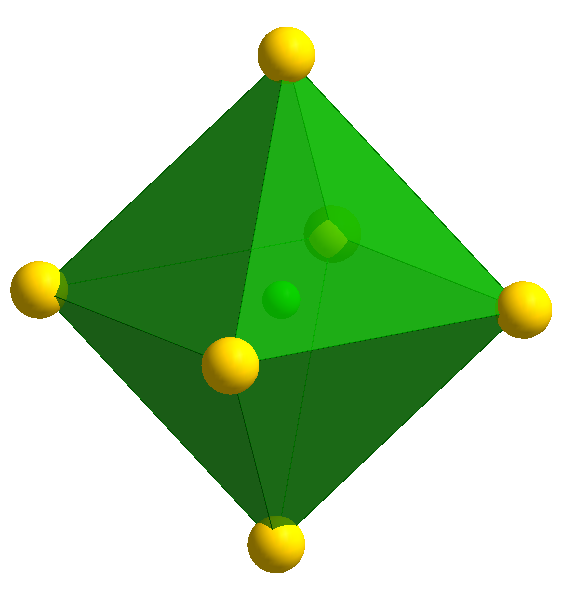
\includegraphics[width=0.4\textwidth]{content/oktaeder}}
  \caption{Gelbe Kugeln in Form eines Oktaeders um eine grüne Kugel. Die Oktaederflächen sind zur Verdeutlichung grün eingefärbt \cite{skript, link}.}
\end{figure}
\newpage
\renewcommand{\thepage}{\roman{page}}\setcounter{page}{1}
\printbibliography
\end{document}4